\documentclass[]{article}
\usepackage{lmodern}
\usepackage{amssymb,amsmath}
\usepackage{ifxetex,ifluatex}
\usepackage{fixltx2e} % provides \textsubscript
\ifnum 0\ifxetex 1\fi\ifluatex 1\fi=0 % if pdftex
  \usepackage[T1]{fontenc}
  \usepackage[utf8]{inputenc}
\else % if luatex or xelatex
  \ifxetex
    \usepackage{mathspec}
  \else
    \usepackage{fontspec}
  \fi
  \defaultfontfeatures{Ligatures=TeX,Scale=MatchLowercase}
\fi
% use upquote if available, for straight quotes in verbatim environments
\IfFileExists{upquote.sty}{\usepackage{upquote}}{}
% use microtype if available
\IfFileExists{microtype.sty}{%
\usepackage{microtype}
\UseMicrotypeSet[protrusion]{basicmath} % disable protrusion for tt fonts
}{}
\usepackage[margin=1in]{geometry}
\usepackage{hyperref}
\hypersetup{unicode=true,
            pdftitle={Pavian Walkthrough},
            pdfauthor={Florian P Breitwieser},
            pdfborder={0 0 0},
            breaklinks=true}
\urlstyle{same}  % don't use monospace font for urls
\usepackage{graphicx,grffile}
\makeatletter
\def\maxwidth{\ifdim\Gin@nat@width>\linewidth\linewidth\else\Gin@nat@width\fi}
\def\maxheight{\ifdim\Gin@nat@height>\textheight\textheight\else\Gin@nat@height\fi}
\makeatother
% Scale images if necessary, so that they will not overflow the page
% margins by default, and it is still possible to overwrite the defaults
% using explicit options in \includegraphics[width, height, ...]{}
\setkeys{Gin}{width=\maxwidth,height=\maxheight,keepaspectratio}
\IfFileExists{parskip.sty}{%
\usepackage{parskip}
}{% else
\setlength{\parindent}{0pt}
\setlength{\parskip}{6pt plus 2pt minus 1pt}
}
\setlength{\emergencystretch}{3em}  % prevent overfull lines
\providecommand{\tightlist}{%
  \setlength{\itemsep}{0pt}\setlength{\parskip}{0pt}}
\setcounter{secnumdepth}{0}
% Redefines (sub)paragraphs to behave more like sections
\ifx\paragraph\undefined\else
\let\oldparagraph\paragraph
\renewcommand{\paragraph}[1]{\oldparagraph{#1}\mbox{}}
\fi
\ifx\subparagraph\undefined\else
\let\oldsubparagraph\subparagraph
\renewcommand{\subparagraph}[1]{\oldsubparagraph{#1}\mbox{}}
\fi

%%% Use protect on footnotes to avoid problems with footnotes in titles
\let\rmarkdownfootnote\footnote%
\def\footnote{\protect\rmarkdownfootnote}

%%% Change title format to be more compact
\usepackage{titling}

% Create subtitle command for use in maketitle
\newcommand{\subtitle}[1]{
  \posttitle{
    \begin{center}\large#1\end{center}
    }
}

\setlength{\droptitle}{-2em}
  \title{Pavian Walkthrough}
  \pretitle{\vspace{\droptitle}\centering\huge}
  \posttitle{\par}
  \author{Florian P Breitwieser}
  \preauthor{\centering\large\emph}
  \postauthor{\par}
  \predate{\centering\large\emph}
  \postdate{\par}
  \date{2017-11-05}


\begin{document}
\maketitle

{
\setcounter{tocdepth}{2}
\tableofcontents
}
\subsection{Introduction}\label{introduction}

Pavian (`pathogen visualization and more') is a interactive web tool to
explore at metagenomics classification results. Pavian has been
developed with this clinical metagenomics in mind. However, it should be
useful to anyone who wants to analyze and visualize their metagenomics
data. This document gives a walkthrough of the interface by looking at
the provided example data from brain biospies. The images have been
generated using RSelenium.

\begin{figure}[htbp]
\centering
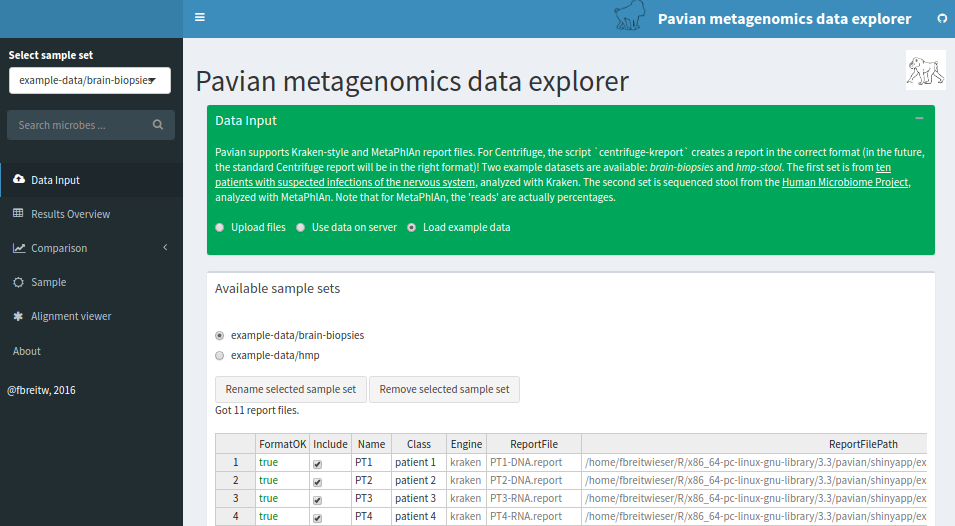
\includegraphics{load-data-set.png}
\caption{Pavian interface with the example data loaded. You can change
the name of the sample set, or the name that appears in the interface
for individual samples. Click `Save table' after any change.}
\end{figure}

\subsection{1) Data Input - Import Kraken and Centrifuge report
files}\label{data-input---import-kraken-and-centrifuge-report-files}

The first step is loading data. Pavian currently supports results from
Kraken (Wood and Salzberg 2014) and Centrifuge (Kim et al. 2016). It
expects files ending with `.report.csv', generated with kraken-report or
centrifuge-report. Before data is loaded, Pavian shows only a limited
part of the interface (see Figure 1). Click `Browse' or `Choose files'
(depending on browser) to select files to upload to Pavian. The uploaded
files will be added to a new sample set with an auto-generated name. You
can change the name of the samples and the sample set using the
interface that appears, once the files are loaded.

In this walk through we use data from Salzberg et al. (2016). To load
this data, click the `Load example data' button. This study sequenced
brain or spinal cord biopsies from 10 patients with suspected central
nervous system (CNS) infections. Upon loading the data, the links to
`Results Overview', `Comparison' and `Sample' become available in the
sidebar, and a table describes the loaded sample set (see Figure 1).

\subsubsection{Brain biopsies data}\label{brain-biopsies-data}

Salzberg et al. (2016) used sequencing to detect the presence of
pathogenic microbes in brain or spinal cord biopsies from 10 patients
with neurological problems indicating possible infection, but for whom
conventional clinical and microbiology studies yielded negative or
inconclusive results. Direct DNA and RNA sequencing of brain tissue
biopsies generated 8.3 million to 29.1 million sequence reads per
sample.

Every samples is from a diseased patient. There are no healthy controls,
and for all but one patient (PT8) there is only one sample available.
The patients had different diseases; thus it was not expected that the
same bug was the cause in the patients. The samples are their own
control - ubiquitously present microbes probably are sequencing or
laboratory contaminants.

The FASTQ files for this study are available at
\url{http://www.ncbi.nlm.nih.gov/bioproject/PRJNA314149}. The reads were
classified with Kraken.

\subsection{2) Results Overview - Look at the overall statistics across
the
samples}\label{results-overview---look-at-the-overall-statistics-across-the-samples}

\begin{figure}[htbp]
\centering
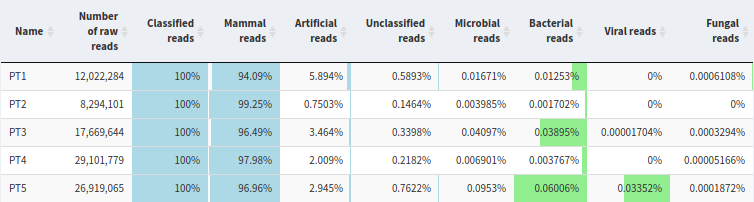
\includegraphics{results-overview.png}
\caption{Results overview gives a quick view to the classification
results.}
\end{figure}

Select `Results Overview' in the sidebar to load the report files. After
the files are loaded, the number of reads in the different samples, as
well as the overall classification in different categories are displayed
in a table (see Figure 2).

The samples of the brain biopsies dataset have between 8.3 and 29
million reads, most of them classified as `mammal' (a `mammal' is
usually the host in these studies). There is a varying number of reads
classified as artificial - usually below 5\%, but two outliers in sample
PT1 and PT7 with 5.9 and 29\%, respectively. The number of reads
classified as microbial is below .1\% in all samples.

\subsection{3) Comparision - Compare the classification across
samples}\label{comparision---compare-the-classification-across-samples}

Click `Comparison' and `All data' to delve into the data (see Figure 3).
The sample comparison view juxtaposes the identification results from
the samples in a query-able table with taxa as rows and samples as
columns. The table provides a visual guide to the values with inline
bars, and the column taxid links to NCBI. You can decide to show
percentages or z-scores, only show results at a certain taxonomic rank,
and filter uninteresting taxa. By default, the taxa `Homo sapiens',
`synthetic construct' and `unclassified' are filtered.

In the brain biopsies dataset, we immediately see an outlier in sample
PT5, which is the only one with a substantial number of JC polyomavirus
reads. Note the table is rather wide with ten samples, and the fourth
column provides an overview of the values in all columns. You can
restrict the view to bacteria, viruses, or eukaryotic microbes by
selecting the appropriate link in the sidebar.

\begin{figure}[htbp]
\centering
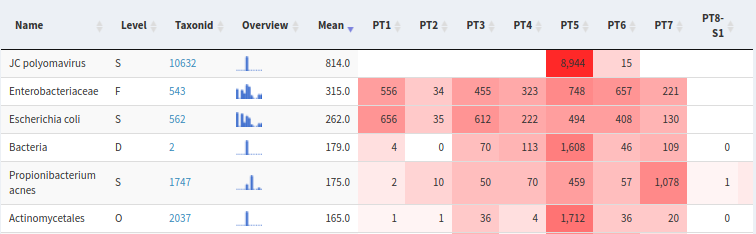
\includegraphics{menu-comp.png}
\caption{Sample comparision provides the data from all the samples in a
sample set in a concise queryable table.}
\end{figure}

\subsection{4) Sample - Zoom into one sample with a Sankey
diagram}\label{sample---zoom-into-one-sample-with-a-sankey-diagram}

As JC Polyomavirus is a prime suspect in sample PT5, let's look further
into the sample. Select `Sample' in the sidebar, and then `PT5' (Figure
5).

\begin{figure}[htbp]
\centering
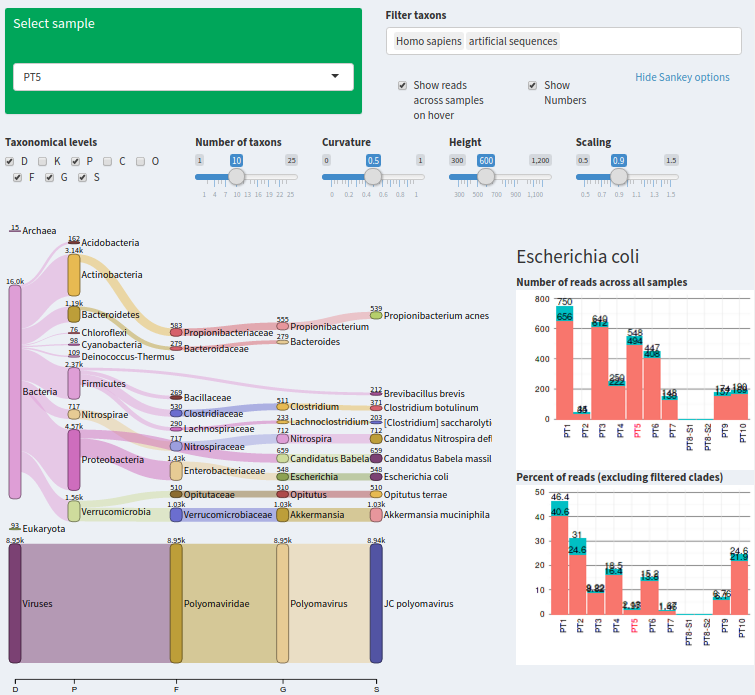
\includegraphics{flow-pt5-2.png}
\caption{Sankey diagram of sample PT5 shows that JC Polyomavirus
dominates the sample, and no other microbiota have been detected in a
significant amount. When hovering nodes, the rea distribution for this
taxon in other samples is displayed on the right. Here, Escherichia coli
is selected.}
\end{figure}

The sample comparison view allows a user to juxtapose the identification
results from multiple samples (Figure 1C). The main view is an
interactive table with taxa as rows and samples as columns. As the
number of samples grows, this table can get very wide; thus to provide
overview of the abundances in wide tables, the third column contains an
inline barchart representation of the counts for a given species (row)
across all samples. By default, read counts at all taxonomy levels are
shown, but it is possible to only show specific taxonomical levels. The
table can be queried and filtered.

The same results may also be inspected with an interactive heatmap,
shown in Figure 1D. The samples and microbes may be clustered to group
together samples with similar microbial profiles. Clicking on a row or
column focuses in on one sample and microbe.

\clearpage

\subsection{5) Alignment viewer - Zoom into one pathogen in one
sample}\label{alignment-viewer---zoom-into-one-pathogen-in-one-sample}

JC polyomavirus has a high read count in sample PT5. However, do these
reads cover the genome, or are they localized in a limited stretch of
the genome? The coverage of the genome can provide a strong indication
whether an assignment is spurious or not. A high read count for a
particular species does not always mean that the microbe is present, as
the reads may map to contaminated regions of a database genome or common
sequences.

Click `Alignment viewer' to get to Pavian's two functionalities to help
in this in-depth investigation. First, it provides a convenient
interface to the NCBI RefSeq assemblies (Kitts et al. 2016) in `Download
genomes for alignment'. There, go to `viral' genome assemblies, and
select `Get assembly info'. Note that every time this is selected, all
the associated assembly summary information from NCBI is downloaded.
After a short while a table appears with all viral RefSeq genome. Search
for `JC Pol' to find the reference genome for this species (see Figure
6). Note that the reference genome is the strain Mad1 originally
uploaded in 1993. Once a row in the table is selected, a link to the
genomic sequence (*\_genomic.fna.gz) is displayed below, as well as
Linux commands to copy and paste for downloading and building an index
based on the genome. Note that the user has to then manually align the
sample sequences and build a BAM file and BAM index.

\begin{figure}[htbp]
\centering
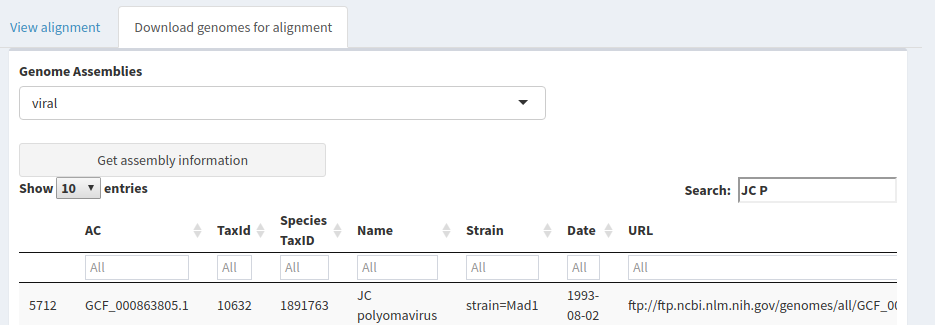
\includegraphics{download-genome-jcv.png}
\caption{Pavian provides an intuitive interface to RefSeq genome
assembly data}
\end{figure}

With a BAM file and BAM index (BAI) available, we can use the genome
viewer. Click `View alignment'. Normally, the two files have to be
uploaded by clicking the `Browse' button. Pavian includes the alignment
of the sequences of PT5 to the reference genome of JC polyomavirus, and
it is loaded by clicking `Show alignment pileup' when no files are
uploaded. Upon loading the files, the coverage over the genome is
displayed (Figure 7). You can select a region to zoom into. For this
genome we see that the reads align pretty randomly across the genome,
but certain small region are not covered. As the reference genome is a
strain that was isolated in 1993, it is very likely that this patient
does have a different strain. Still, the coverage of this genome
provides confidence that it is the same species.

\begin{figure}[htbp]
\centering
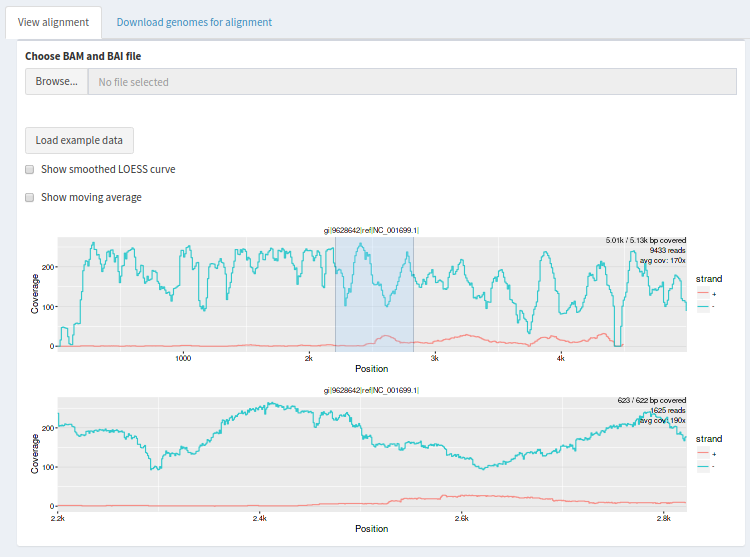
\includegraphics{alignment-viewer-pt5.png}
\caption{The alignment of the reads of sample PT5 to JC polyomavirus
reference genome can be explored with the alignment viewer. There is a
high coverage of most regions of the genome.}
\end{figure}

\clearpage

\subsection*{References}\label{references}
\addcontentsline{toc}{subsection}{References}

\hypertarget{refs}{}
\hypertarget{ref-DKim_SSalzber2016-Biorxiv}{}
Kim, Daehwan, Li Song, Florian P Breitwieser, and Steven L Salzberg.
2016. ``Centrifuge: Rapid and Sensitive Classification of Metagenomic
Sequences.'' \emph{Genome Research}. Cold Spring Harbor Labs Journals.
doi:\href{https://doi.org/10.1101/054965}{10.1101/054965}.

\hypertarget{ref-PKitts_AKimchi2016-NAR}{}
Kitts, Paul A., Deanna M. Church, Françoise Thibaud-Nissen, Jinna Choi,
Vichet Hem, Victor Sapojnikov, Robert G. Smith, et al. 2016. ``Assembly:
A Resource for Assembled Genomes at Ncbi.'' \emph{Nucleic Acids Res} 44
(D1). National Center for Biotechnology Information, National Library of
Medicine, National Institutes of Health, Bethesda, MD 20894, USA.:
D73--D80.
doi:\href{https://doi.org/10.1093/nar/gkv1226}{10.1093/nar/gkv1226}.

\hypertarget{ref-SSalzberg_CPardo2016-NNN}{}
Salzberg, Steven L., Florian P. Breitwieser, Anupama Kumar, Haiping Hao,
Peter Burger, Fausto J. Rodriguez, Michael Lim, et al. 2016.
``Next-Generation Sequencing in Neuropathologic Diagnosis of Infections
of the Nervous System.'' \emph{Neurol Neuroimmunol Neuroinflamm} 3 (4).
ter Science,; Biostatistics (S.L.S.), Johns Hopkins University,
Baltimore, MD.: e251.
doi:\href{https://doi.org/10.1212/NXI.0000000000000251}{10.1212/NXI.0000000000000251}.

\hypertarget{ref-DWood_SSalzberg2014-GB}{}
Wood, Derrick E., and Steven L. Salzberg. 2014. ``Kraken: Ultrafast
Metagenomic Sequence Classification Using Exact Alignments.''
\emph{Genome Biol} 15 (3): R46.
doi:\href{https://doi.org/10.1186/gb-2014-15-3-r46}{10.1186/gb-2014-15-3-r46}.


\end{document}
